\section{Integralrechnung}
\subsection{Berechnung}
$\int \alpha f(x) + \beta g(x)\,dx = \alpha \int f(x)\,dx + \beta \int g(x)\,dx$

\subsubsection{Substitutionsregel}
$\int F'(g(x)) g'(x)dx = F(g(x))$


\begin{enumerate}
	\item Für die neue Variable $u = g(x)$ bildet man: $\frac{du}{dx} = g'(x)
	\Leftrightarrow du = g'(x)dx$. Ersetzt also $g(x) = u$ und $dx =
	\frac{du}{g'(x)}$. Wenn noch $x$ übrig sind, ist ein Zwischenschritt nötig:
	Löse $u = g(x)$ durch $x = h(x)$ nach $x$ auf und ersetze die restlichen $x$
	durch $h(x)$.
	\item Bei bestimmten Integralen: Sei $\int_a^b \ldots \,dx$. Dann sind die neuen
	Grenzen für das neue Integral $g(a)$ und $g(b)$
	\item Berechne das Integral in $u$
	\item Ersetze im Ergebnis $u$ durch $g(x)$
\end{enumerate}

\paragraph{Beispiel 1}
Das Integral $\int_{-2}^1 x^2 \,dx$ berechnet die blaue Fläche die durch die Funktion $f(x) = x^2$ beschränkt wird.
$F(x)$ sei die Stammfunktion von $f(x)$,  generell berechnen wir $\int x^y \,dx = \frac{x^{(y+1)}}{y+1}$, somit $F(x) = \frac{x^3}{3}$.
Somit $\int_{-2}^1 x^2 \,dx = F(x) \left |_{-2}^1 \right. = F(1) - F(-2) =  \frac{1^3}{3} -  \frac{-2^3}{3} = \frac{1}{3} +  \frac{8}{3} = 3.$

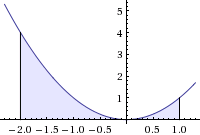
\includegraphics[scale=1]{integral_x2.png}

\paragraph{Beispiel 2}
$\int_0^2 x \sqrt{x+1}^3 \,dx$

Die Wurzel wird substituiert: $u = g(x) = \sqrt{x+1}$.

\begin{enumerate}
	\item $\frac{du}{dx} = g'(x) = \frac{1}{2\sqrt{x+1}} = \frac{1}{2u}$. Somit
	wird $\sqrt{x+1}^3$ durch $u^3$ ersetzt und $dx$ durch
	$\frac{du}{\frac{1}{2}u} = 2u\,du$. Im Integral wären somit die Wurzel und das
	$dx$ ersetzt. Es bleibt noch das $x$ übrig vor der Wurzel. Lösen wird
	$\sqrt{x+1} = u$ nach $x$ auf, so erhalten wir $x = u^2 - 1$.
	\item Neue Grenzen: $g(0) = 1$ und $g(2) = \sqrt{3}$
	\item $\int_0^2 x \sqrt{x+1}^3 \,dx = \int_1^{\sqrt{3}} (u^2 - 1)u^3 2u \,du =
	2\int(u^6 -u^4) \,du = [\frac{2}{7}u^7 - \frac{2}{5}u^5]_{1}^{\sqrt{3}}$
	\item Rücksubstitution: $\int_0^2 x \sqrt{x+1}^3 \,dx =
	[\frac{2}{7}\sqrt{x+1}^7 - \frac{2}{5}\sqrt{x+1}^5]_{1}^{\sqrt{3}} = \ldots = \frac{144}{35}\sqrt{3} +
	\frac{4}{35}$
\end{enumerate}